%============================================================
%  Xiamen University Malaysia Article Template
%  Compile with XeLaTeX or LuaLaTeX to ensure Times New Roman
%============================================================
\documentclass[12pt]{article}

%------------------------------------------------------------
% Packages
%------------------------------------------------------------
\usepackage{fontspec}      % For Times New Roman
\usepackage{setspace}      % For line spacing
\usepackage{geometry}      % Page margins
\usepackage{fancyhdr}      % Header & footer
\usepackage{titlesec}      % Custom headings
\usepackage{csquotes}      % Quotation tools (optional)
\usepackage{listings}
\usepackage{xcolor} 
\usepackage{float}
\usepackage{indentfirst}
\usepackage{graphicx}
\usepackage[colorlinks=true, linkcolor=blue, urlcolor=blue,citecolor=black]{hyperref}
\usepackage[backend=biber,style=apa]{biblatex}
\addbibresource{references.bib}  % 不要加 .bib 扩展名


%------------------------------------------------------------
% Fonts & Spacing
%------------------------------------------------------------
\setmainfont{Times New Roman}
\setstretch{1.5}           % 1.5 line spacing

%------------------------------------------------------------
% Geometry (1‑inch margins by default)
%------------------------------------------------------------
\geometry{a4paper, margin=1in}

%代码格式
\lstnewenvironment{python}[1][]
{
	\lstset{
		language=Python,
		basicstyle=\ttfamily\small,
		numbers=left,
		numberstyle=\tiny\color{gray},
		numbersep=8pt,            % 数字到文字之间 2pt
		frame=single,
		framesep=2pt,             % 框线内四周都留 2pt
		xleftmargin=0pt,          % 整个框紧贴正文左边距
		framexleftmargin=2pt,     % 框线内左侧到文字 2pt
		backgroundcolor=\color[RGB]{245,245,245},
		breaklines=true,
		breakindent=10pt,
		keywordstyle=\color[RGB]{255,119,0},
		morekeywords={as, self},
		deletekeywords={print},
		keywordstyle=[2]\color[RGB]{144,0,144},
		morekeywords=[2]{print},
		stringstyle=\color[RGB]{0,170,0},
		commentstyle=\color[RGB]{221,0,0},
		showstringspaces=false,
		#1
	}
}{}


%------------------------------------------------------------
% Header & Footer
%------------------------------------------------------------
\pagestyle{fancy}
\fancyhf{}                              % Clear default header/footer
\fancyhead[C]{XIAMEN UNIVERSITY MALAYSIA} % Centered header text
\fancyfoot[C]{\thepage}                % Centered page number
\renewcommand{\headrulewidth}{0pt}      % Remove header line

%------------------------------------------------------------
% Title & Section Formatting (14‑pt Times New Roman, bold)
%------------------------------------------------------------
\titleformat{\section}
{\fontsize{14pt}{16pt}\selectfont\bfseries}
{\thesection}{1em}{}

\titleformat{\subsection}
{\fontsize{14pt}{16pt}\selectfont\bfseries}
{\thesubsection}{1em}{}

% Optional: adjust subsubsection as “subtitle” too
\titleformat{\subsubsection}
{\fontsize{14pt}{16pt}\selectfont\bfseries}
{\thesubsubsection}{1em}{}

% Ensure normal text stays 12‑pt Times New Roman (set by documentclass)

%------------------------------------------------------------
% Document begins
%------------------------------------------------------------
\begin{document}
	
	% ----------------- Main Content ----------------------------
	
	% Example Title (remove if not needed)
	%\section*{Sample Document Title}
	%\addcontentsline{toc}{section}{Sample Document Title}
	
	\section{Introduction}
	%为什么没有缩进。。。。
	With the recent renewal of the MBTI's popularity, posts or analyses about it have become widespread on public platforms. It seems that MBTI has become a way people use at first meetings.
	
	The Myers-Briggs Type Indicator (MBTI) is a psychological framework primarily used to describe and measure personality traits by categorizing individuals into four dichotomous dimensions. In essence, it aims to reflect how people perceive the world and make decisions based on their internal experiences(\cite{yang2022research}).
	
	And the test is conducted through asking a series of questions, and the type of question is kind of like asking about the tendency to do something. Based on the responses, individuals receive a result represented by four letters, each corresponding to one of the four bipolar dimensions. According to \textcite{boyle1995mbti}, these four dichotomous dimensions classify individuals as either extraverted (E) or introverted (I), sensing (S) or intuitive (N), thinking (T) or feeling (F), and judging (J) or perceiving (P). Combinations of the four preferences generate one of 16 personality types (e.g., ESFJ, ENFP, INTP, ISFJ), each associated with distinct behavioral tendencies, reflecting differences in attitudes, orientation, and decision-making styles. Also, on the official website, it will provide the future career options for you, like INFP, which may be more suitable for being an author. The percentage of each standard will also show in the final result.
	
	The MBTI provides a widely recognized and accessible way to understand personality, making it a useful foundation for further behavioral and data-driven analysis.
	
	\section{Objective}
	\begin{enumerate} 
		\item Evaluate the reliability of the MBTI from a statistical perspective.    \item Explore the potential application of MBTI in social media behavior analysis.    
		\item Help people better understand personality traits and behavioral patterns.    
		\item Helping people eliminate stereotypes caused by MBTI personality types.
	\end{enumerate}
	
	\section{Problem Statements}
	\begin{enumerate}
		\item Are the results of the MBTI personality test statistically robust and reliable?
		\item Do the four dimensions of MBTI work independently, or are they connected in some way?
		\item Do people with different MBTI types have different levels of activity on the internet?
		\item Do significant differences exist in the interest preferences and behavioral patterns of different MBTI personality types on social networking sites?
	\end{enumerate}
	
	\section{Data Collection}
	\begin{enumerate}
		\item “MBTI Personality Type Twitter Dataset”
		
		Tweets were originally harvested from the public Twitter API by a third-party collector and later released on Kaggle by Mazlumi(\url{https://www.kaggle.com/datasets/mazlumi/mbti-personality-type-twitter-dataset})
		\begin{itemize}
			\item 8,600 Twitter users, and 1 million raw tweets.
			\item Each user record contains the self-declared MBTI type (e.g., “ENFP”) taken from the user’s bio.
			\item The text has not been further cleaned or filtered—URLs, emojis, hashtags, and retweets remain. Researchers must therefore perform their preprocessing (tokenisation, stop-word removal, emoji handling, etc.) before analysis.    
		\end{itemize}
		\item “KPMIRU Questionnaires Data”
		
		Questionnaire responses compiled and shared on Kaggle by Pmenshih(\url{https://www.kaggle.com/datasets/pmenshih/kpmiru-questionnaires-data})
		\begin{itemize}
			\item Contains every participant’s item-level answers to the full KPMIRU personality inventory (several dozen Likert-scale questions).
			\item Provides the scored results for all four MBTI dimensions—reported as continuous scores (0–100 per axis) as well as the final type label (e.g., “ISTJ”).
			\item Demographic fields (age range, gender, education) are included, enabling richer statistical controls. 
		\end{itemize}
		
		Together, the Twitter dataset supplies large-scale, real-world language samples with self-reported types, while the KPMIRU dataset offers clean, psychometrically scored questionnaire data. The two sources complement each other for training and validating our emotion-aware MBTI models.
	\end{enumerate}
	\begin{figure}[H]
		\centering
		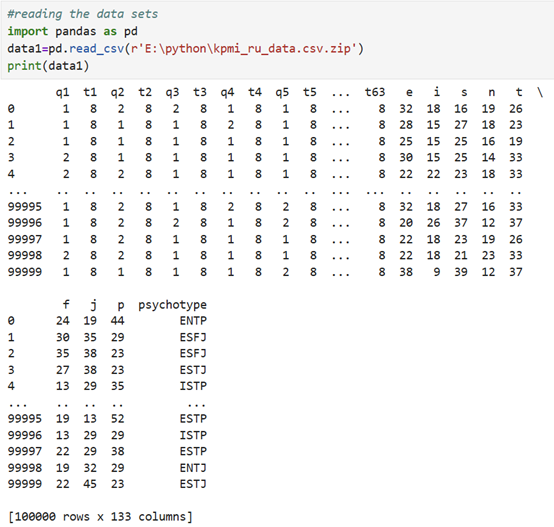
\includegraphics{Q1P1} %这个图片怎么这么糊啊(┬┬﹏┬┬),到时候让csq重新截图给我
		\caption{reading data sets}
	
	\end{figure}
	\begin{figure}[H]
		\centering
		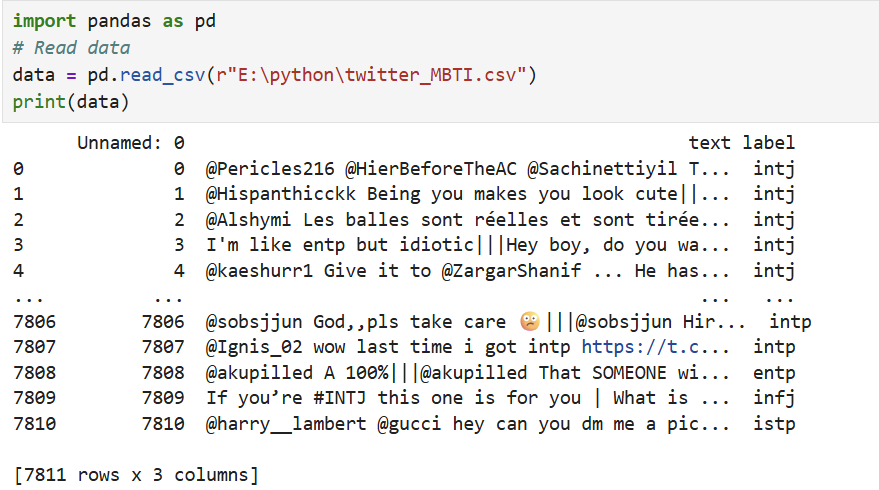
\includegraphics[width=0.9\textwidth]{Q1P2}
		
	\end{figure}
	As illustrated in the two Figures above, the combined Kaggle sources provide information on:
	\begin{enumerate}
		\item Self-reported MBTI types for each respondent
		\item Raw Twitter posts and basic tweet metadata linked to those MBTI labels  
		\item Demographic and psychometric questionnaire answers (KPMIRU survey) 
		\item Behavioral metrics such as posting frequency and topic keywords extracted from the tweets
	\end{enumerate}
	
	\section{Data Cleaning and Pre-processing}
	\subsection{Handling Missing Values}
	\begin{enumerate}
		\item We use dropna() to eliminate any records with missing or null entries. Fortunately, the dataset had no missing psychotype labels or scoring data.
			\begin{figure}[H]
			\centering
			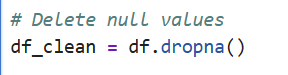
\includegraphics[width=0.9\textwidth]{Q1P4}
			
		\end{figure}
	\end{enumerate}
	\subsection{Outlier Detection and Correction}
	\begin{enumerate}
		\item Outliers in numeric scores were identified using the IQR (interquartile range) method.
		\item For each numeric column, we computed Q1, Q3. IQR = Q3 - Q1 represent the middle 50\% of the data distribution. The lower\_bound and upper\_bound represent the boundaries of the normal range under the Interquartile Range (IQR) rule. And then we replaced values outside [Q1 − 1.5×IQR, Q3 + 1.5×IQR] with the column median. 
		\item The median substitution method mainly serves to stabilize the overall distribution and avoid the influence of extreme values.
		\begin{figure}[H]
			\centering
			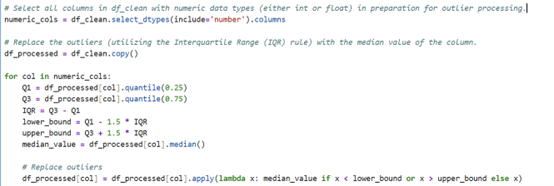
\includegraphics[width=0.9\textwidth]{Q1P5}
			
		\end{figure}
	\end{enumerate}
	\subsection{Export the cleaned data}
	After completing the outlier replacement and data cleaning process, we used df.info() to verify the integrity and structure of the cleaned dataset. The cleaned DataFrame was then exported using the to\_csv() method, which saved it as kpmi\_ru\_data(Cleaned).csv for downstream analysis. The index=False parameter ensured that row indices were not written to the CSV file.
	\begin{figure}[H]
		\centering
		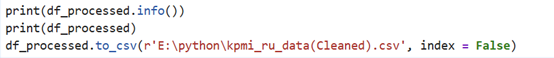
\includegraphics[width=0.9\textwidth]{Q1P6}
		
	\end{figure}
	\begin{figure}[H]
		\centering
		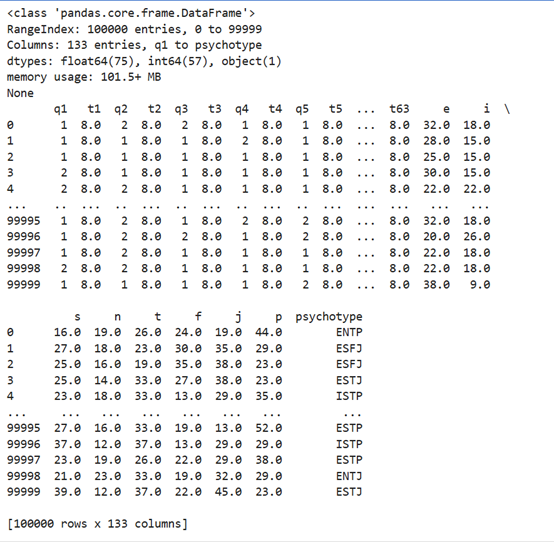
\includegraphics[width=0.9\textwidth]{Q1P7}
		
	\end{figure}
	The data in the figure 3.1 is the data after our data cleaning.
	
	\section{Model Building and Evaluation}
	Chi-square test is an on parametric statistical test to determine if the two or more classifications of the samples are independent or not\cite{zibran2007chi}. We all know that MBTI has four dimensions(Extraversion–Introversion (E–I), Sensing–Intuition (S–N), Thinking–Feeling (T–F) and Judging–Perceiving (J–P)). But whether or not these four dimensions interrelated or independent of each other stays unknown. For explanation, let’s consider the data presented in Figure 3.1 which comprising 100 000 respondents, providing information on the scoring fields of the four dimensions of MBTI. In order to find the answer, we use the chi-square test.
	
	Each respondent’s type label (e.g., ENTP) was decomposed into its four constituent letters, and the sample was cross-classified into a 2 × 2 × 2 × 2 contingency table (16 cells)(shown in figure 3.2) 
	\begin{figure}[H]
		\centering
		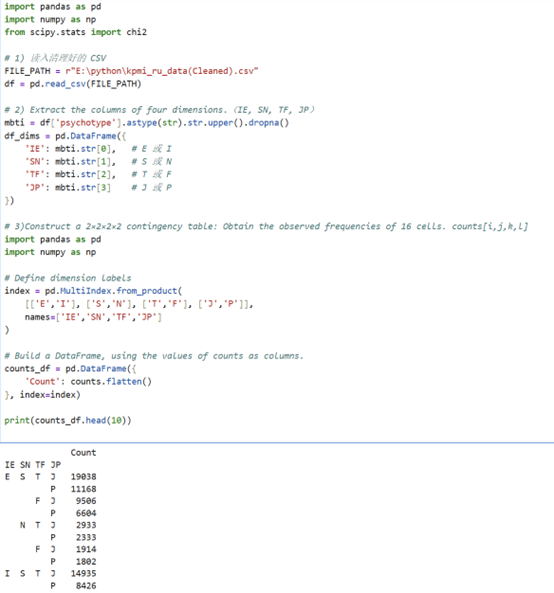
\includegraphics[width=0.9\textwidth]{Q1P8}
		
	\end{figure}
	Then we calculate the marginal distribution (the distribution of each dimension separately), for example, N\_IE = [count(E), count(I)](shown in figure3.3)
	\begin{figure}[H]
		\centering
		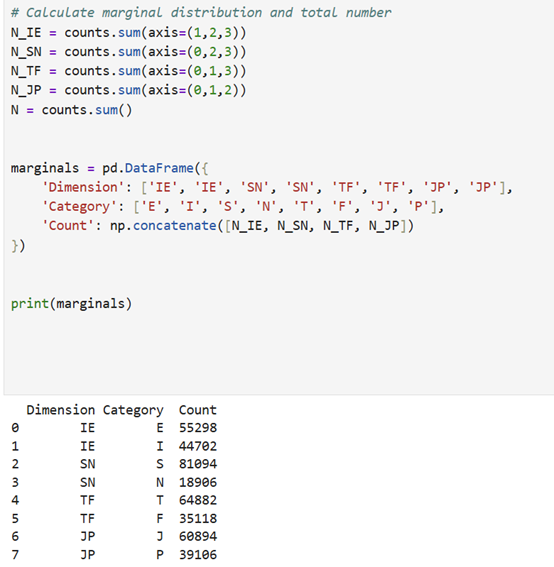
\includegraphics[width=0.9\textwidth]{Q1P9}
		
	\end{figure}
	Under the null hypothesis of mutual independence, the expected frequency in each cell was computed as the product of the four one-dimensional marginal distributions multiplied by the sample size.(shown in figure3.4)
	\begin{figure}[H]
		\centering
		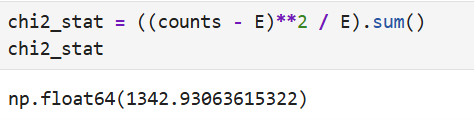
\includegraphics[width=0.9\textwidth]{Q1P10}
		
	\end{figure}
	Now, it’s time to calculate the Pearson chi-square statistic, while O is observed value and E is expected value.(shown in figure 3.5)
	\[
	\chi^2 = \sum \frac{(O - E)^2}{E}
	\]
	\begin{figure}[H]
		\centering
		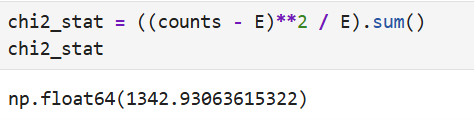
\includegraphics[width=0.9\textwidth]{Q1P10}
		
	\end{figure}
	Finally, with χ² = 1342.93 and df = 11,we can compute the right - tailed probability corresponding to the chi - square statistic under 10 degrees of freedom, which is 0(shown in figure 3.6). Because the p-value falls far below the conventional α =0.05 threshold, the null hypothesis is decisively rejected: the observed joint distribution of MBTI preferences deviates dramatically from what would be expected if the four indices varied independently. In practical terms, substantial associations exist among the E–I, S–N, T–F and J–P scales, corroborating earlier psychometric critiques that the MBTI dimensions are not orthogonal factors but overlap to a non-trivial extent. Actually, some researchers had also proven that the four dimensions of MBTI are not independent. \textcite{fleenor1997relationship} investigated the intercorrelations among MBTI continuous scores and found that while most dimension pairs demonstrated relatively low correlations, the correlation between the Sensing–Intuition (SN) and Judging–Perceiving (JP) scales was notably higher. Specifically, the study reported a correlation coefficient of r = 0.41 between SN and JP, indicating a moderate positive relationship. This finding has been replicated in other research and suggests that individuals who prefer intuition are more likely to also prefer perceiving. As such, the assumption of strict statistical independence between MBTI preference axes, particularly between SN and JP, may not hold, which is in line with the findings of our study.
	\begin{figure}[H]
		\centering
		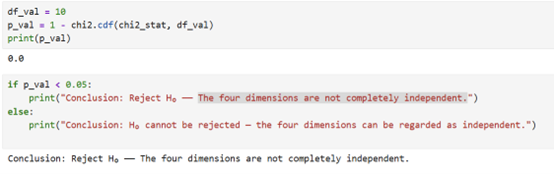
\includegraphics[width=0.9\textwidth]{Q1P11}
		
	\end{figure}
	
	\section{Exploratory Data Analysis (EDA)}
	\subsection{Data Visualization}
	\subsubsection{MBTI Type Frequency}
	\begin{figure}[H]
		\centering
		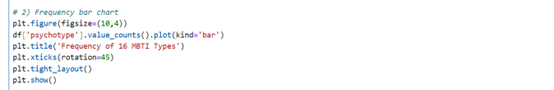
\includegraphics[width=0.9\textwidth]{Q1P3EDA1}
		
	\end{figure}
	
	A frequency bar chart of the 16 MBTI types was generated using the value\_counts() function on the psychotype column. The result was plotted using matplotlib and is shown in Figure 4.1.1.
	%后面需要统一图片命名!!
	\begin{figure}[H]
		\centering
		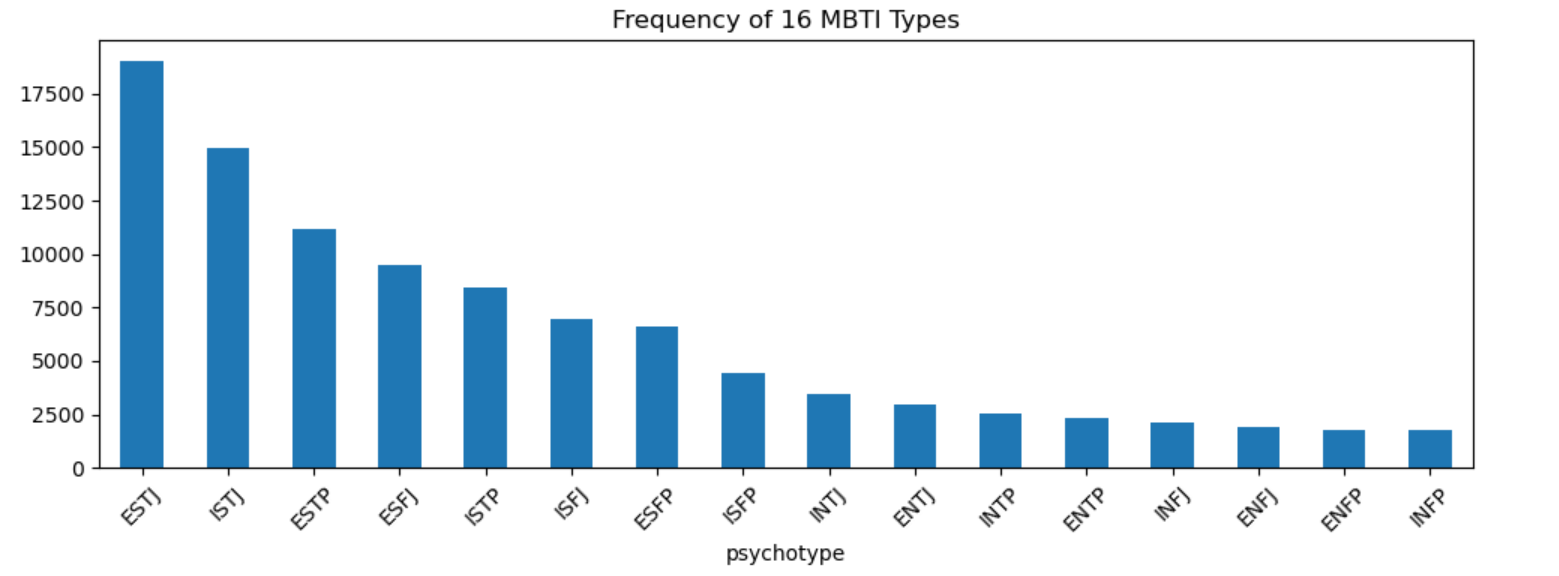
\includegraphics{Q1EDA2} 
		\caption{Frequency of 16 MBTI Types}		
	\end{figure}
	
	As seen in Figure 4.1.1 above, the frequency of 16 MBTI types has been shown in a descending order. The type ESTJ ranks first, which shows that, based on our dataset, the proportion of ESTJ people is the highest. Conversely, the proportion of INFP people is the lowest. Additionally, it can be observed that the \_S\_J people rankings are relatively high in frequency, as the \_NF\_ people rankings are relatively low.
	
	Also, Figure 4.1.1 exhibits severe right oblique imbalance distribution, as the number of ESTJ people is nearly nine times as many as the number of INFP people. This phenomenon may be attributed to our database being originally from Kaggle, and certain MBTI type tends to participate in such investigations.
	
	This contrasts with national MBTI distribution statistics reported in the MBTI® Manual, where ISFJ and ESFJ were found to be the most common types among U.S. adults (Myers et al., 1998), suggesting that our dataset, to a certain extent, fits the population-level trends. In distinct regions, the regional differences may influence MBTI type distributions in specific rankings.
	
	\subsubsection{MBTI Type Frequency}
		\begin{figure}[H]
		\centering
		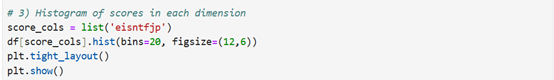
\includegraphics[width=0.9\textwidth]{Q1EDA3}
		
	\end{figure}
	
	Histograms of scores in each MBTI dimension were generated using pandas.DataFrame.hist and visualized with matplotlib as shown in Figure 4.1.2.
	\begin{figure}[H]
		\centering
		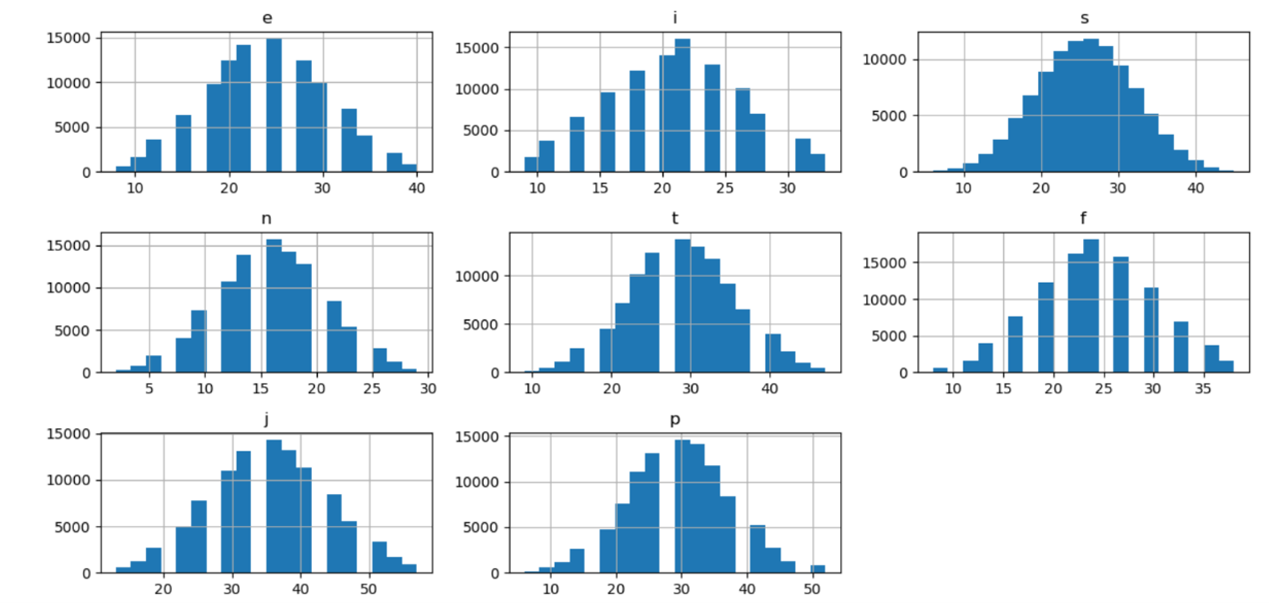
\includegraphics{Q1EDA4} 
		\caption{Histogram of MBTI Dimension Scores}		
	\end{figure}
	
	As seen in Figure 4.1.2 above, from the score concentration trend, the eight MBTI poles vary in concentration. For example, E, S, and T scores are generally spread from 10 to 40, while N and I scores are more narrowly concentrated between 5 to 30. And in detail, in the dimension of P and T, exhibit higher scores, which shows the preference toward Thinking and Perceiving. Compared to them, in the dimension of N and I, they exhibit lower scores, which indicates most people are more inclined toward Extraversion and Sensing.
	
	From the data obtained from these diagrams, we can observe that most samples in these dimensions show distributional asymmetries, as not evenly distributed. Particularly for the high values of J and low values of N, this result matches the observation at 4.1.1 that \_S\_J types dominate the database.
	
	\subsubsection{MBTI Type Frequency}
	\subsubsection{MBTI Type Frequency}
	\begin{figure}[H]
	\centering
	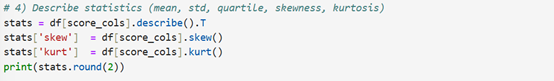
\includegraphics[width=0.9\textwidth]{Q1EDA5}
	
	\end{figure}	
	
	Descriptive statistics of each MBTI dimension were computed and consolidated into a single summary table, including skewness and kurtosis, to facilitate score distribution analysis shown in Table 4.1.1
	%这里table要改!!
	\begin{figure}[H]
		\centering
		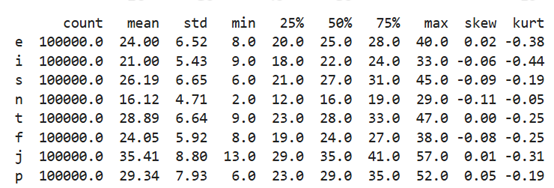
\includegraphics{Q1EDA6} 
		\caption{Descriptive Statistics of MBTI Dimension Scores}		
	\end{figure}
	
	%还有交叉引用要改(不过是不是不改也行?	
	Based on Table 4.1.3, it can be observed that the dimensions of I, S, N, and F showcase a notable positive skew distribution, as the dimension of N, with a value of -0.11, demonstrates left skewness most. This phenomenon tends to show that most people are more likely to be Sensing(S) and so on. And in contrast, the dimension of P with the value of +0.05 exhibits right skewness, implying a preference towards lower values, showing that Judging(J) dominates more in this database. Results of these also support the conclusion in Figure 4.1.1 that \_S\_J people occupy the majority.
	
	And from the kurtosis value, it can be seen that most values are around 0 and negative, which suggests that all the dimension is distributed platykurtic. With relatively concentrated values, this exhibits the loss of extreme outliers. Also, the maximum value and minimum value that all dimensions have can be used in the form of Max-Min, which demonstrates that J and P dimensions have the largest difference, indicating that individual differences between them are the strongest.
	\begin{figure}[H]
		\centering
		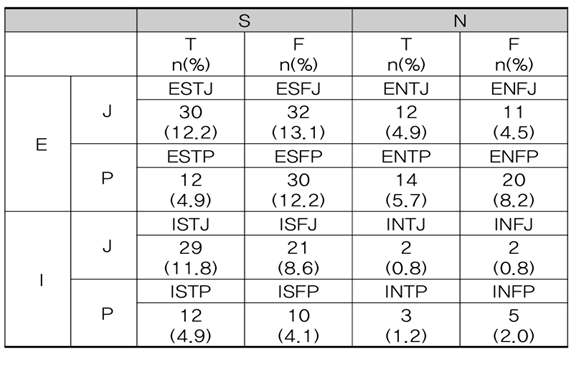
\includegraphics{Q1EDA7} 
		\caption{MBTI Distribution of 16 Personality Types}		
	\end{figure}
	
	Figure 4.1.3 MBTI Distribution of 16 Personality Types from Jang and Kim (2014), supporting the dominance of \_S\_J types observed in our dataset. 
	
	\subsubsection{MBTI Type Frequency}
	\begin{figure}[H]
		\centering
		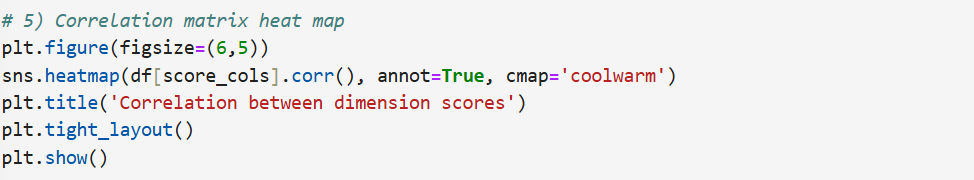
\includegraphics[width=0.9\textwidth]{Q1EDA8}
		
	\end{figure}	
	A Pearson correlation heatmap was constructed to visualize linear relationships among MBTI dimension scores, as shown in Figure 4.1.4.
	\begin{figure}[H]
		\centering
		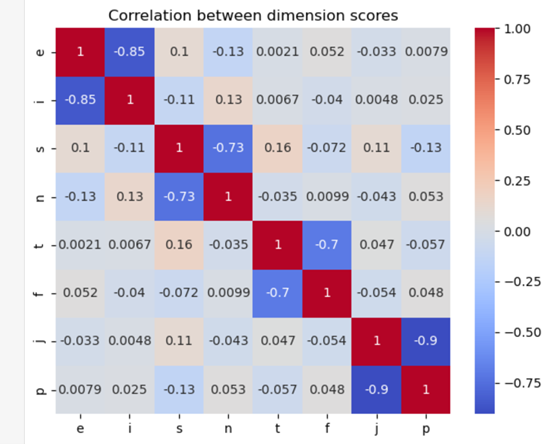
\includegraphics{Q1EDA9} 
		\caption{Correlation Heatmap of MBTI Dimension Scores}		
	\end{figure}
	
	As seen in Figure 4.1.4 above, the correlation between the opposite dimensions, like E vs I, S vs N, T vs F, and J vs P. All of them are strongly negative, which is consistent with the design concept of MBTI, as the two poles of each dimension are opposed. As a result, the MBTI method has its rationality. This result aligns with (Li et al., 2024), who also observed that “the correlations between the four axes are generally weak, indicating that the personality traits on each axis are relatively independent” (p. 12).
	
	Furthermore, in Figure 4.1.4, the correlation between other dimension pairs is low are nearly 0. This phenomenon supports that the dimensions are seemingly independent. While the correlation between S and T is +0.16, a bit larger than others, it indicates that someone who is Sensing(S) tends to be Thinking(T). In contrast, the correlation between S and P is -0.13, which indicates that those who are Sensing(S) tend to be Judging(J).
	%先综述主题建模是什么——》数据清洗步骤必要性解释,结果展示-》主题建模步骤-》EDA
	%intro需要解释objective的原因,将文章分为两个分析方向,解释两者之间的联系;MBTI的进一步解释有必要,写什么根据我后面EDA决定
	\section{EDA}
	
	
	\subsection{Sample Equation}
	Here is a displayed equation for illustration:
	\[
	E = mc^{2}
	\]
	
	\section{Method}
	Continue writing your content here.
	\begin{python}
def quicksort(arr):
if len(arr) <= 1:
return arr
pivot = arr[0]
left = [x for x in arr[1:] if x < pivot]
right = [x for x in arr[1:] if x >= pivot]
return quicksort(left) + [pivot] + quicksort(right)
	\end{python}
	
	


% ----------------- References ------------------------------

\printbibliography[title={References}]

\end{document}
